\chapter{Introduction}
\label{chap:introduction}
\section{Motivation}
%and Background??

%The background of the study will discuss your problem statement, rationale, and research questions. It links introduction to your research topic and ensures a logical flow of ideas.  Thus, it helps readers understand your reasons for conducting the study.
%HER MÅ JEG OGSÅ HA MED AT SOM NEVNT I ABSTRACT??, MÅ VI GJENNOM FLERE STEG. NESTE STEG ER Å DESIGNE EN SENSORBÆRENDE PLATFORM SOM KAN BRUKE DETEKSJONSMETODENE. 

%http://ec.europa.eu/environment/marine/good-environmental-status/descriptor-10/pdf/GESAMP_microplastics%20full%20study.pdf

Today, the applications for plastics are huge, making the material popular worldwide. %335 million metric tons of plastic was produced in 2016. %(https://www.statista.com/statistics/282732/global-production-of-plastics-since-1950/)
% https://www.darrinqualman.com/global-plastics-production/
Approximately 400 million metric tons of plastic is produced yearly, and the production is projected to nearly double within the next 10-15 years. %https://wedocs.unep.org/bitstream/handle/20.500.11822/25398/WED%20Messaging%20Two-Page%2027April.pdf?sequence=12&isAllowed=y
In addition to being a strong, light and inexpensive material, the different types of plastic cover an almost full-scaled spread of needs. High electrical isolation properties are useful in one area, while durable and strong material can be ideal in other areas. What do we read of this? Plastics have incredibly useful and versatile properties. However, this worldwide spread of plastics holds a significant side effect. 
\\\\
The different types of plastic have polymer structures that make the material almost non-biodegradable. In addition, the structures of plastics can hold additives. This is initially something that can be utilized, as additives can be incorporated in order to give the plastic a desired property. Typically additives are fire retardants, stabilizers, antibiotics, pigments etc. %[https://www.darrinqualman.com/global-plastics-production/]
Problems arise when the additives that blend into the pieces of plastics, turns out to be toxins and the plastic debris serves as a vector, introducing toxic elements into the ecosystem. As this vector is not biodegradable, it can travel between ecosystems as an immortal catalyst.
\\\\
The largest source of microplastic is the discharge of larger plastic pieces gradually fragmented into smaller plastic debris. The fragmentation occurs due to wear and tear from the environment. The biggest cause of decomposition is UV radiation from the sun. The rays provide oxidative decomposition of polymers, which in turn will give weak and brittle plastic debris. At this state, mechanical forces can easily fragment the weak plastic piece. Of such forces wind, waves and human activity are good examples. The state of a large plastic piece floating around the many seas can thereby quickly result in many smaller pieces and in turn be fragmented to microplastic. In addition, wind and currents will bring the microplastic away from its initial point of outlet, leaving the microplastic widely spread. 
\\\\
%https://setac.onlinelibrary.wiley.com/doi/10.1002/ieam.5630030412
The largest issue with microplastic is due to ingestion by marine biota. Once microplastic is ingested, it is in most cases retained in the digestive system or absorbed by the intestines. After a while, the plastic debris are stored in organs and tissue. Due to the fact that plastics are not biodegradable, the chemicals will hardly be excreted by the organism ingesting the piece, but rather accumulate. This is called bioaccumulation. 
\\\\
%https://www.sciencedirect.com/science/article/pii/S0160412017322298 
Bioaccumulation creates the foundation of biomagnification, causing the poisoning of entire food chains. Organisms and animals placed at a higher trophic level are often in need of a larger amount of food than what the species on a lower level can serve. This consumption need means that the concentrated bioaccumulation is even larger at higher trophic levels. In fact, the concentration of an environmental toxicity increases with each level of the food chain - in turn affecting human beings as well. This is called biomagnification. 
\\\
Microplastic can be confused with phyto-plankton. This is especially inconvenient as the phyto-plankton creates the basis of all biomass production in the ocean. Phyto-plankton is eaten by the zoo-plankton, which again is food to larger organisms. One of the most common types of microplastic, polystyrene, can often be mistaken for phyto-plankton. This is tragic, as an intake of polystyrene could come with a series of negative consequences. %(http://www.pnas.org/content/113/9/2430).
\\\\
An example of a typical bioaccumulated chemical, traveling through trophic levels, is Polychlorinated biphenyls (PCBs), a group of manmade chemicals. Ryan et al. (1988) proved that PCB in the bird's tissue originates from plastic particles.(*) Sadly PCBs are harmful chemicals, even in very low amounts. The ingestion of PCB, for instance through a zoo-plankton containing PCB-loaded microplastics, can cause reproductive disorders, change the hormone levels and increase the risk of several diseases. In some cases, an intake can lead to death. %[(Ryan et al., 1988, Lee et al., 2001)].
\\\\
Furthermore, some types of bacteria are attracted to free floating marine debris. These are better known as “hitch hikers”, and can threaten sensitive coastal environments, as the bacteria are far from their natural habitats. 
%(Environmental implications of plastic debris in marine settings-entanglement, ingestion, smothering, hangers-on, hitch-hiking and alien invasions Murray R. Gregory)
\\\\
Different types of plastic have different densities. Some types have higher density than water and float, while other types are denser than water. This contributes to the fact that plastic can be found throughout the entire ocean column, and is present in many ecosystems(*). As a result, plastic debris have impacted more than 690 marine. Small particles of plastic have been observed in the digestive tract of organisms from different trophic levels. 
\\\\
While microplastics does damages as a toxic carrying vector, larger pieces of plastics can act as a physical threat in other ways. Polyethylene bags, operating in the ocean currents, have a large resemblance to the predators targeted by turtles. (*) Plastic debris can thus prevent their survival %(Bugoni et al., 2001, Duguy et al., 1998).
The ingestion of larger plastic debris can, among other things, reduce food intake, cause internal damage, strangling or even death after blockage of the intestinal tract. %(Zitko and Hanlon, 1991).
\\\\
Marine biological diversity is already exposed to climate change, over-fishing and other man-made disruptions. As if this were not enough, plastic pollution, with more than 8 billion kilograms entering the ocean annually
%[http://www3.weforum.org/docs/WEF_The_New_Plastics_Economy.pdf],
also causes huge damage to the marine environment. (*)
%* = The pollution of the marine environment by plastic debris: a review Jose G.B. Derraik *

\subsection{Taking Action}
Now that the large impact of plastic is clear, methods on how to reduce this impact are in order. A good way to work with materials, identify them or learn about their properties, is to study how light interacts with them - spectroscopy. By definition spectroscopy examines how light behaves in the target and recognizes materials based on their different spectral signatures. This can be identified from the spectrum, describing the amount of light in different wavelengths, showing how much light is reflected, emitted and transmitted from the target. In other words, the spectrum simply shows how much of a certain color the light contains. 
\\\\
Spectral signatures can be thought of as fingerprints. While fingerprints often is used to identify a person, spectral signatures can be used to identify materials. One of the purposes of this study, is to identify different types of plastic using their spectral signatures. %A thought: As different types of plastic are composed by different polymer structure accepting additives in various degree, one might be able to identify the plastic types most resistant to additives
\\\\
%Development of hyperspectral imaging as a bio-optical taxonomic tool for pigmented marine organisms - geir
Former studies conducted on marine organisms, show that reflectance signatures, obtained from an underwater hyperspectral imager, are related to the absorption signature of that specific organism. %(Volent et al. 2007, 2009)
\\\\
The research questions driving this project are centered around whether microplastics and their spectral signatures in fact can be separated from other material and microorganisms. Do different types of plastics leave different spectral signatures? Could a signature change as the sea tears the plastic pieces? Is it possible that the spectral signatures differ in different environments?
\\\\
\section{Research Question}
The latter questions are important to address when detecting and inspecting microplastic in the ocean. This thesis will dive deeper into some of these questions, in particularly one question; Do different types of plastics obtain different spectral signatures within visual light?
\\\\
\section{Main Contributions - kladd} This paragraph is currently a placeholder. In this section the breaking results will be described in short (elevator pitch). This result could be why [result] is in particularly suitable when detecting microplastic.
\\\\
(If moving passed the spectra of visual light, the wavelengths are too large to penetrate the water as wanted. When the waves propagate with a very high frequency, the light cannot go through water as desired. Therefore, the visual light spectra is a constraint when looking at the resulting signatures). NO, we cannot separate the different types of plastic based on their spectral signature. However, when testing with other organisms, a clear clustering is presented. The challenge is that in order to classify the plastics, the rest of the material or organisms in the image needs to be classified - (method of elimination). 
\\\\
\section{Thesis Outline}
%denne kan vel være i preface eller noe?
The work supporting this thesis is three-folded. In order to achieve relevant and precise knowledge, a literature study was conducted. This study involved research on both specific methods and technology used, and what has been done in general. The research regarding these topics were done mainly through researching a bunch of scientific papers. However, even with the most recent publications, there are still research done - not yet published. The second part of this thesis was therefore to travel around Trondheim meeting with the experts. During exciting meetings with Emlyn Davies, Andy M. Booth, Geir Johnsen, Aksel Alstad Mogstad, Bert van Bavel, Asgeir J. S{\o}rensen and Albert Van Oyen(from now on referred to as "the experts"), new knowledge was acquired. After this, the problem description finally took form. Through planning with the experts, the experiment description were formed. These experiments represent the third and last part of the three-folded work. 

\todo[inline, color=orange!40]{Burde jeg heller si dette i preface?}

%Hva alle kapittelene handler om

\begin{figure}
  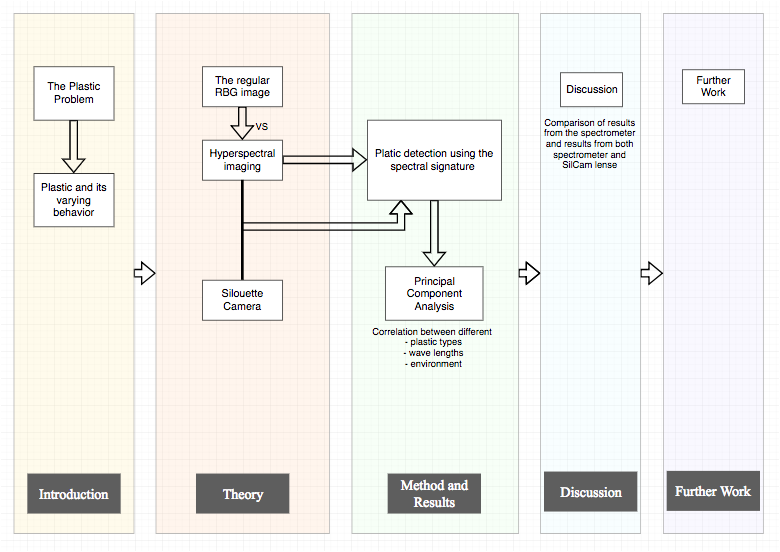
\includegraphics[width=\linewidth]{Images/outline.png}
  \caption{Thesis Outline, roughly sketched}
  \label{fig:outline}
\end{figure}

